\documentclass[landscape]{article}
\usepackage[a4paper, margin=2cm]{geometry}
\usepackage{tikz}
\usetikzlibrary{shapes,arrows,positioning,fit,backgrounds,calc,shadows}

\begin{document}

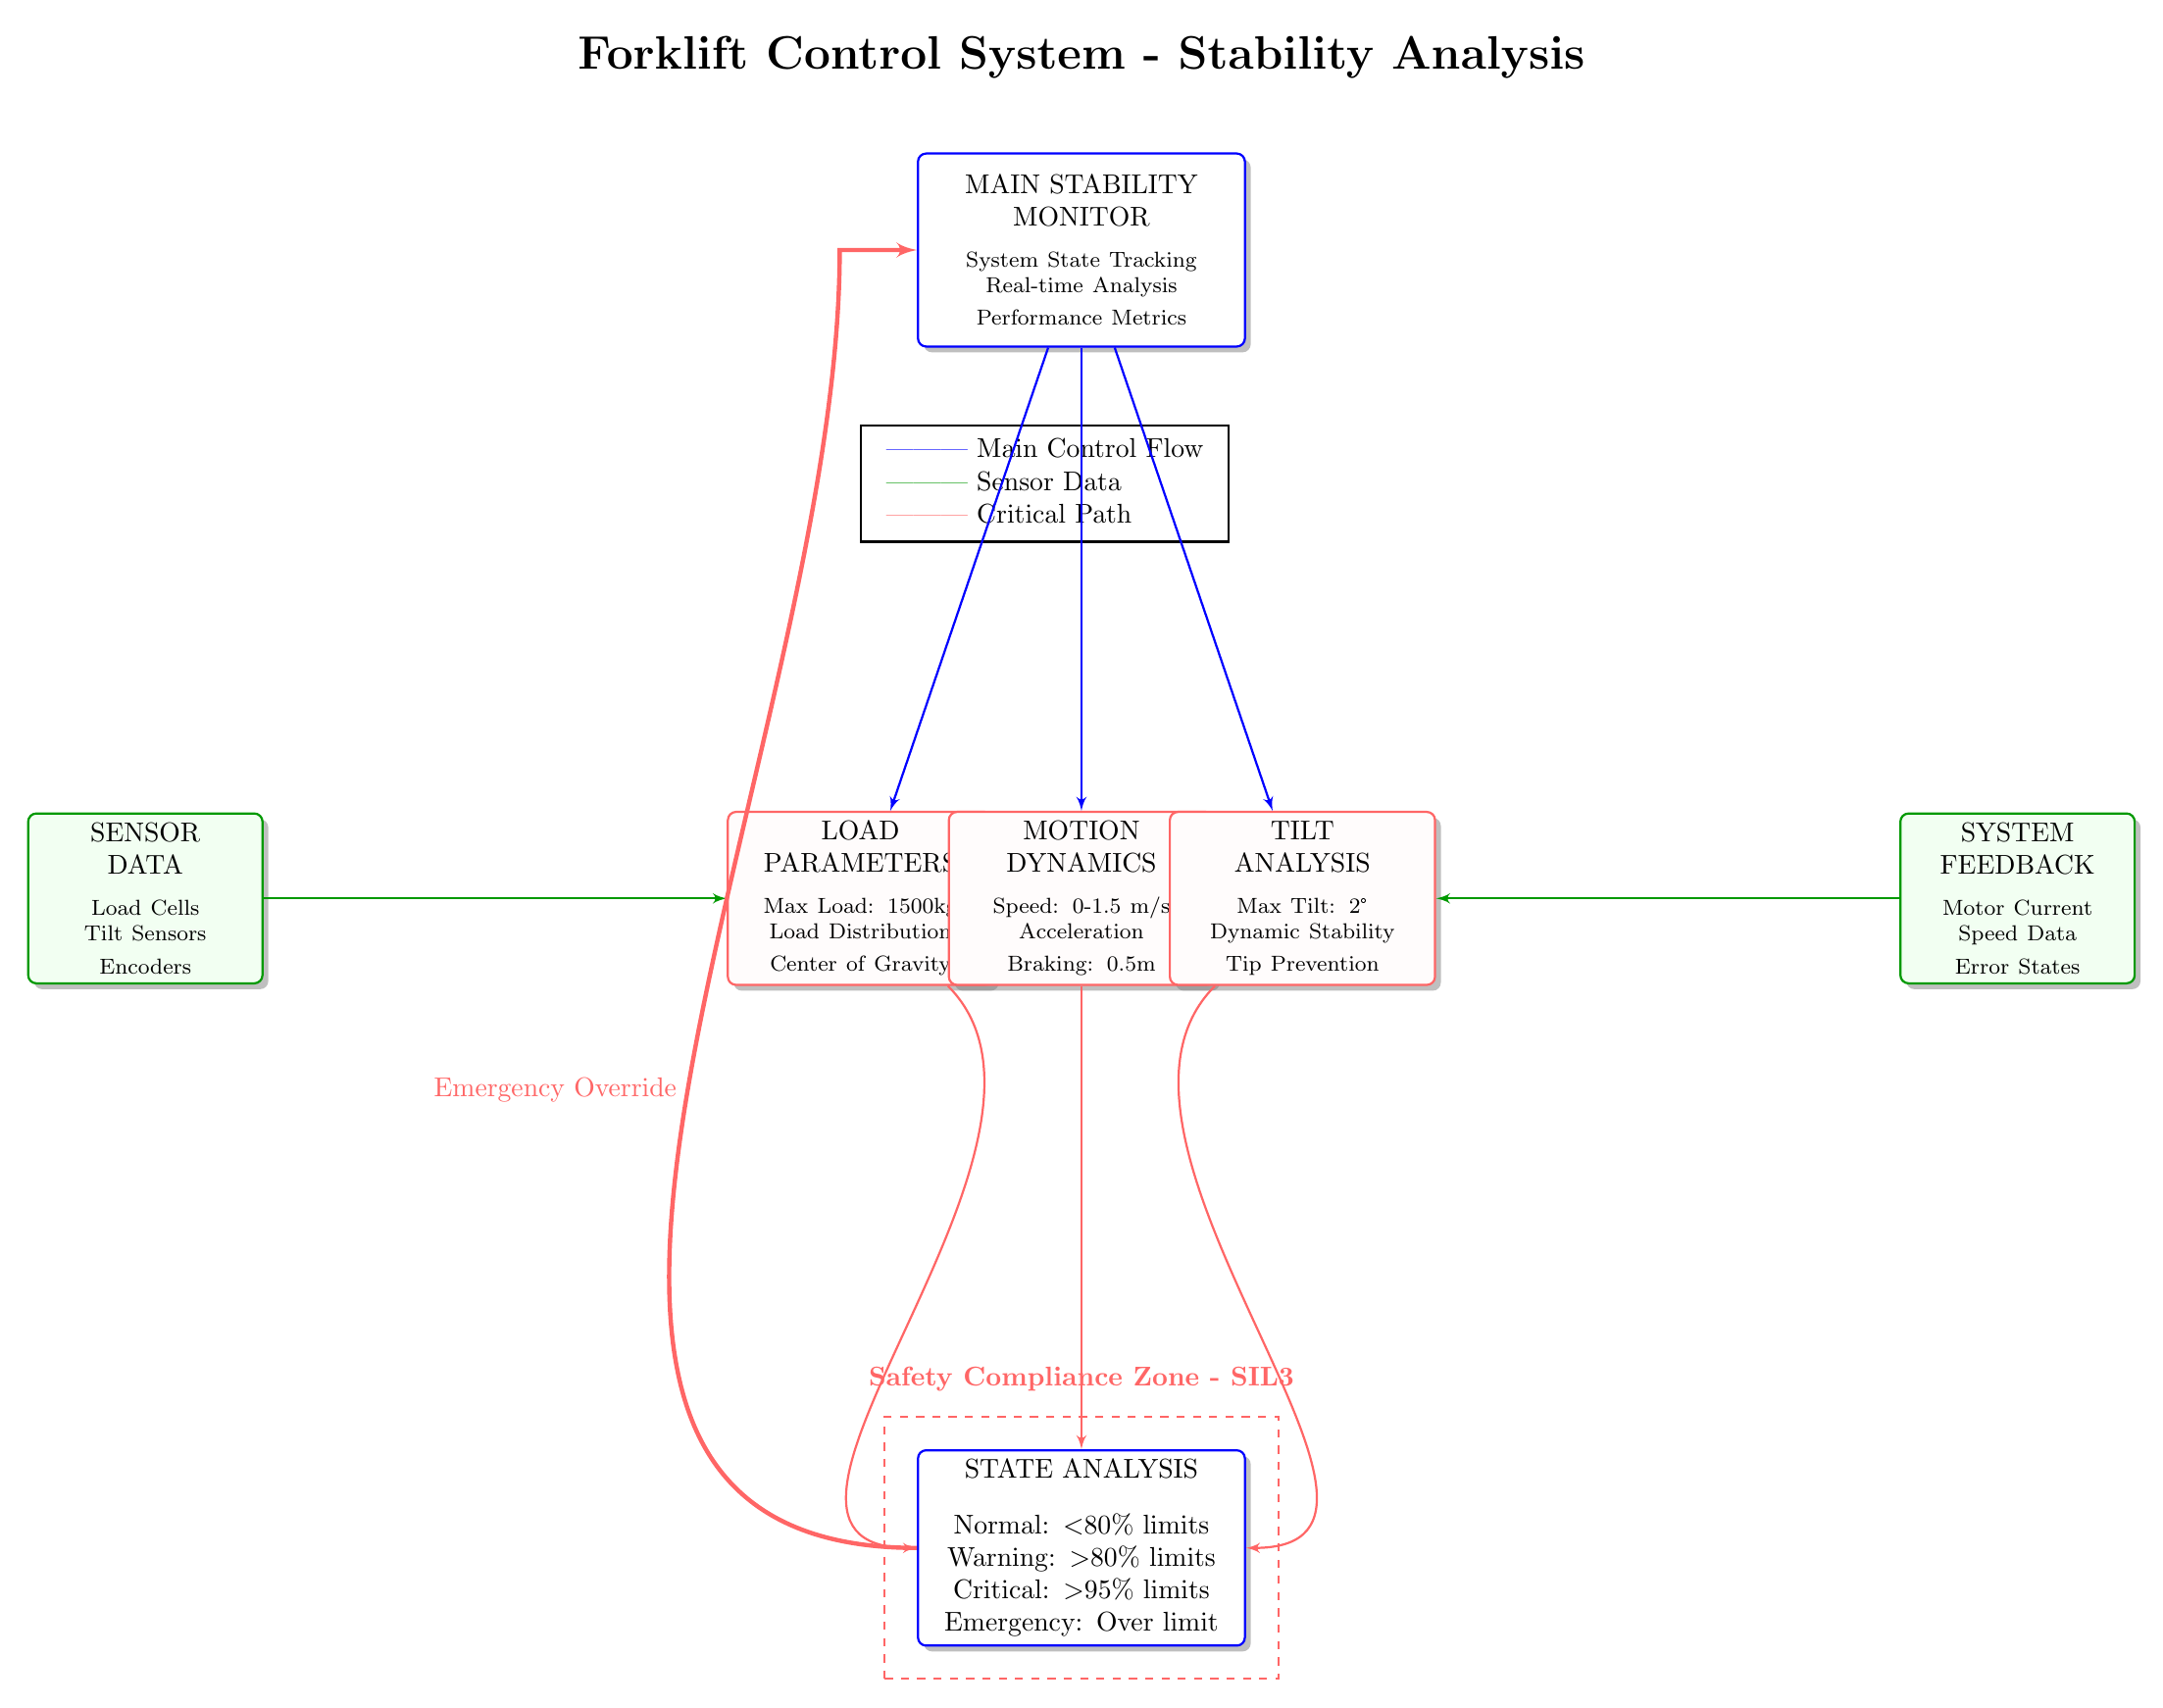
\begin{tikzpicture}[
    auto,
    mainblock/.style={
        rectangle,
        draw=blue,
        thick,
        text width=4cm,
        minimum height=2.5cm,
        align=center,
        rounded corners=3pt,
        fill=white,
        drop shadow
    },
    sensorblock/.style={
        rectangle,
        draw=green!60!black,
        thick,
        text width=2.8cm,
        minimum height=2.2cm,
        align=center,
        rounded corners=3pt,
        fill=green!5,
        drop shadow
    },
    paramblock/.style={
        rectangle,
        draw=red!60,
        thick,
        text width=3.2cm,
        minimum height=2.2cm,
        align=center,
        rounded corners=3pt,
        fill=pink!5,
        drop shadow
    },
    line/.style={draw=blue, thick, -latex'},
    sensor line/.style={draw=green!60!black, thick, -latex'},
    critical line/.style={draw=red!60, thick, -latex'}
]

% Title
\node [font=\LARGE\bfseries] at (0,6) {Forklift Control System - Stability Analysis};

% Main Stability Monitor
\node [mainblock] (monitor) at (0,3.5) {MAIN STABILITY\\MONITOR\\[0.2cm]
    \footnotesize
    System State Tracking\\
    Real-time Analysis\\
    Performance Metrics};

% Parameter Blocks with increased spacing
\node [paramblock, below left=6cm and -1cm of monitor] (load) {LOAD\\PARAMETERS\\[0.2cm]
    \footnotesize
    Max Load: 1500kg\\
    Load Distribution\\
    Center of Gravity};

\node [paramblock, below=6cm of monitor] (motion) {MOTION\\DYNAMICS\\[0.2cm]
    \footnotesize
    Speed: 0-1.5 m/s\\
    Acceleration\\
    Braking: 0.5m};

\node [paramblock, below right=6cm and -1cm of monitor] (tilt) {TILT\\ANALYSIS\\[0.2cm]
    \footnotesize
    Max Tilt: 2°\\
    Dynamic Stability\\
    Tip Prevention};

% Sensor and Feedback Blocks with increased spacing
\node [sensorblock, left=6cm of load] (sensors) {SENSOR\\DATA\\[0.2cm]
    \footnotesize
    Load Cells\\
    Tilt Sensors\\
    Encoders};

\node [sensorblock, right=6cm of tilt] (feedback) {SYSTEM\\FEEDBACK\\[0.2cm]
    \footnotesize
    Motor Current\\
    Speed Data\\
    Error States};

% State Analysis Block
\node [mainblock, below=6cm of motion] (state) {STATE ANALYSIS\\[0.3cm]
    Normal: {$<$}80\% limits\\
    Warning: {$>$}80\% limits\\
    Critical: {$>$}95\% limits\\
    Emergency: Over limit};

% Safety Box with more padding
\begin{scope}[on background layer]
    \node[draw=red!60, thick, dashed, fit={($(state.north west)+(-0.3,0.3)$) ($(state.south east)+(0.3,-0.3)$)}] 
        (safety_box) {};
    \node[above=0.2cm of safety_box.north] {\color{red!60}\textbf{Safety Compliance Zone - SIL3}};
\end{scope}

% Legend with better positioning
\node[draw, thick, fill=white, below right=1cm and -5cm of monitor] {
    \begin{tabular}{ll}
        \textcolor{blue}{―――} Main Control Flow\\
        \textcolor{green!60!black}{―――} Sensor Data\\
        \textcolor{red!60}{―――} Critical Path
    \end{tabular}
};

% Connections with smoother paths
\draw [line] (monitor) -- (load);
\draw [line] (monitor) -- (motion);
\draw [line] (monitor) -- (tilt);
\draw [sensor line] (sensors) -- (load);
\draw [sensor line] (feedback) -- (tilt);
\draw [critical line] (load) to[out=-45, in=180] (state);
\draw [critical line] (motion) -- (state);
\draw [critical line] (tilt) to[out=-135, in=0] (state);

% Emergency Override with smoother curve
\draw [critical line, ultra thick] (state.west) to[out=180, in=-90] 
    node[left, text=red!60] {Emergency Override} 
    ($(monitor.west) + (-1,0)$) -- (monitor.west);

\end{tikzpicture}

\end{document} 